\documentclass[1p]{elsarticle_modified}
%\bibliographystyle{elsarticle-num}

%\usepackage[colorlinks]{hyperref}
%\usepackage{abbrmath_seonhwa} %\Abb, \Ascr, \Acal ,\Abf, \Afrak
\usepackage{amsfonts}
\usepackage{amssymb}
\usepackage{amsmath}
\usepackage{amsthm}
\usepackage{scalefnt}
\usepackage{amsbsy}
\usepackage{kotex}
\usepackage{caption}
\usepackage{subfig}
\usepackage{color}
\usepackage{graphicx}
\usepackage{xcolor} %% white, black, red, green, blue, cyan, magenta, yellow
\usepackage{float}
\usepackage{setspace}
\usepackage{hyperref}

\usepackage{tikz}
\usetikzlibrary{arrows}

\usepackage{multirow}
\usepackage{array} % fixed length table
\usepackage{hhline}

%%%%%%%%%%%%%%%%%%%%%
\makeatletter
\renewcommand*\env@matrix[1][\arraystretch]{%
	\edef\arraystretch{#1}%
	\hskip -\arraycolsep
	\let\@ifnextchar\new@ifnextchar
	\array{*\c@MaxMatrixCols c}}
\makeatother %https://tex.stackexchange.com/questions/14071/how-can-i-increase-the-line-spacing-in-a-matrix
%%%%%%%%%%%%%%%

\usepackage[normalem]{ulem}

\newcommand{\msout}[1]{\ifmmode\text{\sout{\ensuremath{#1}}}\else\sout{#1}\fi}
%SOURCE: \msout is \stkout macro in https://tex.stackexchange.com/questions/20609/strikeout-in-math-mode

\newcommand{\cancel}[1]{
	\ifmmode
	{\color{red}\msout{#1}}
	\else
	{\color{red}\sout{#1}}
	\fi
}

\newcommand{\add}[1]{
	{\color{blue}\uwave{#1}}
}

\newcommand{\replace}[2]{
	\ifmmode
	{\color{red}\msout{#1}}{\color{blue}\uwave{#2}}
	\else
	{\color{red}\sout{#1}}{\color{blue}\uwave{#2}}
	\fi
}

\newcommand{\Sol}{\mathcal{S}} %segment
\newcommand{\D}{D} %diagram
\newcommand{\A}{\mathcal{A}} %arc


%%%%%%%%%%%%%%%%%%%%%%%%%%%%%5 test

\def\sl{\operatorname{\textup{SL}}(2,\Cbb)}
\def\psl{\operatorname{\textup{PSL}}(2,\Cbb)}
\def\quan{\mkern 1mu \triangleright \mkern 1mu}

\theoremstyle{definition}
\newtheorem{thm}{Theorem}[section]
\newtheorem{prop}[thm]{Proposition}
\newtheorem{lem}[thm]{Lemma}
\newtheorem{ques}[thm]{Question}
\newtheorem{cor}[thm]{Corollary}
\newtheorem{defn}[thm]{Definition}
\newtheorem{exam}[thm]{Example}
\newtheorem{rmk}[thm]{Remark}
\newtheorem{alg}[thm]{Algorithm}

\newcommand{\I}{\sqrt{-1}}
\begin{document}

%\begin{frontmatter}
%
%\title{Boundary parabolic representations of knots up to 8 crossings}
%
%%% Group authors per affiliation:
%\author{Yunhi Cho} 
%\address{Department of Mathematics, University of Seoul, Seoul, Korea}
%\ead{yhcho@uos.ac.kr}
%
%
%\author{Seonhwa Kim} %\fnref{s_kim}}
%\address{Center for Geometry and Physics, Institute for Basic Science, Pohang, 37673, Korea}
%\ead{ryeona17@ibs.re.kr}
%
%\author{Hyuk Kim}
%\address{Department of Mathematical Sciences, Seoul National University, Seoul 08826, Korea}
%\ead{hyukkim@snu.ac.kr}
%
%\author{Seokbeom Yoon}
%\address{Department of Mathematical Sciences, Seoul National University, Seoul, 08826,  Korea}
%\ead{sbyoon15@snu.ac.kr}
%
%\begin{abstract}
%We find all boundary parabolic representation of knots up to 8 crossings.
%
%\end{abstract}
%\begin{keyword}
%    \MSC[2010] 57M25 
%\end{keyword}
%
%\end{frontmatter}

%\linenumbers
%\tableofcontents
%
\newcommand\colored[1]{\textcolor{white}{\rule[-0.35ex]{0.8em}{1.4ex}}\kern-0.8em\color{red} #1}%
%\newcommand\colored[1]{\textcolor{white}{ #1}\kern-2.17ex	\textcolor{white}{ #1}\kern-1.81ex	\textcolor{white}{ #1}\kern-2.15ex\color{red}#1	}

{\Large $\underline{11n_{15}~(K11n_{15})}$}

\setlength{\tabcolsep}{10pt}
\renewcommand{\arraystretch}{1.6}
\vspace{1cm}\begin{tabular}{m{100pt}>{\centering\arraybackslash}m{274pt}}
\multirow{5}{120pt}{
	\centering
	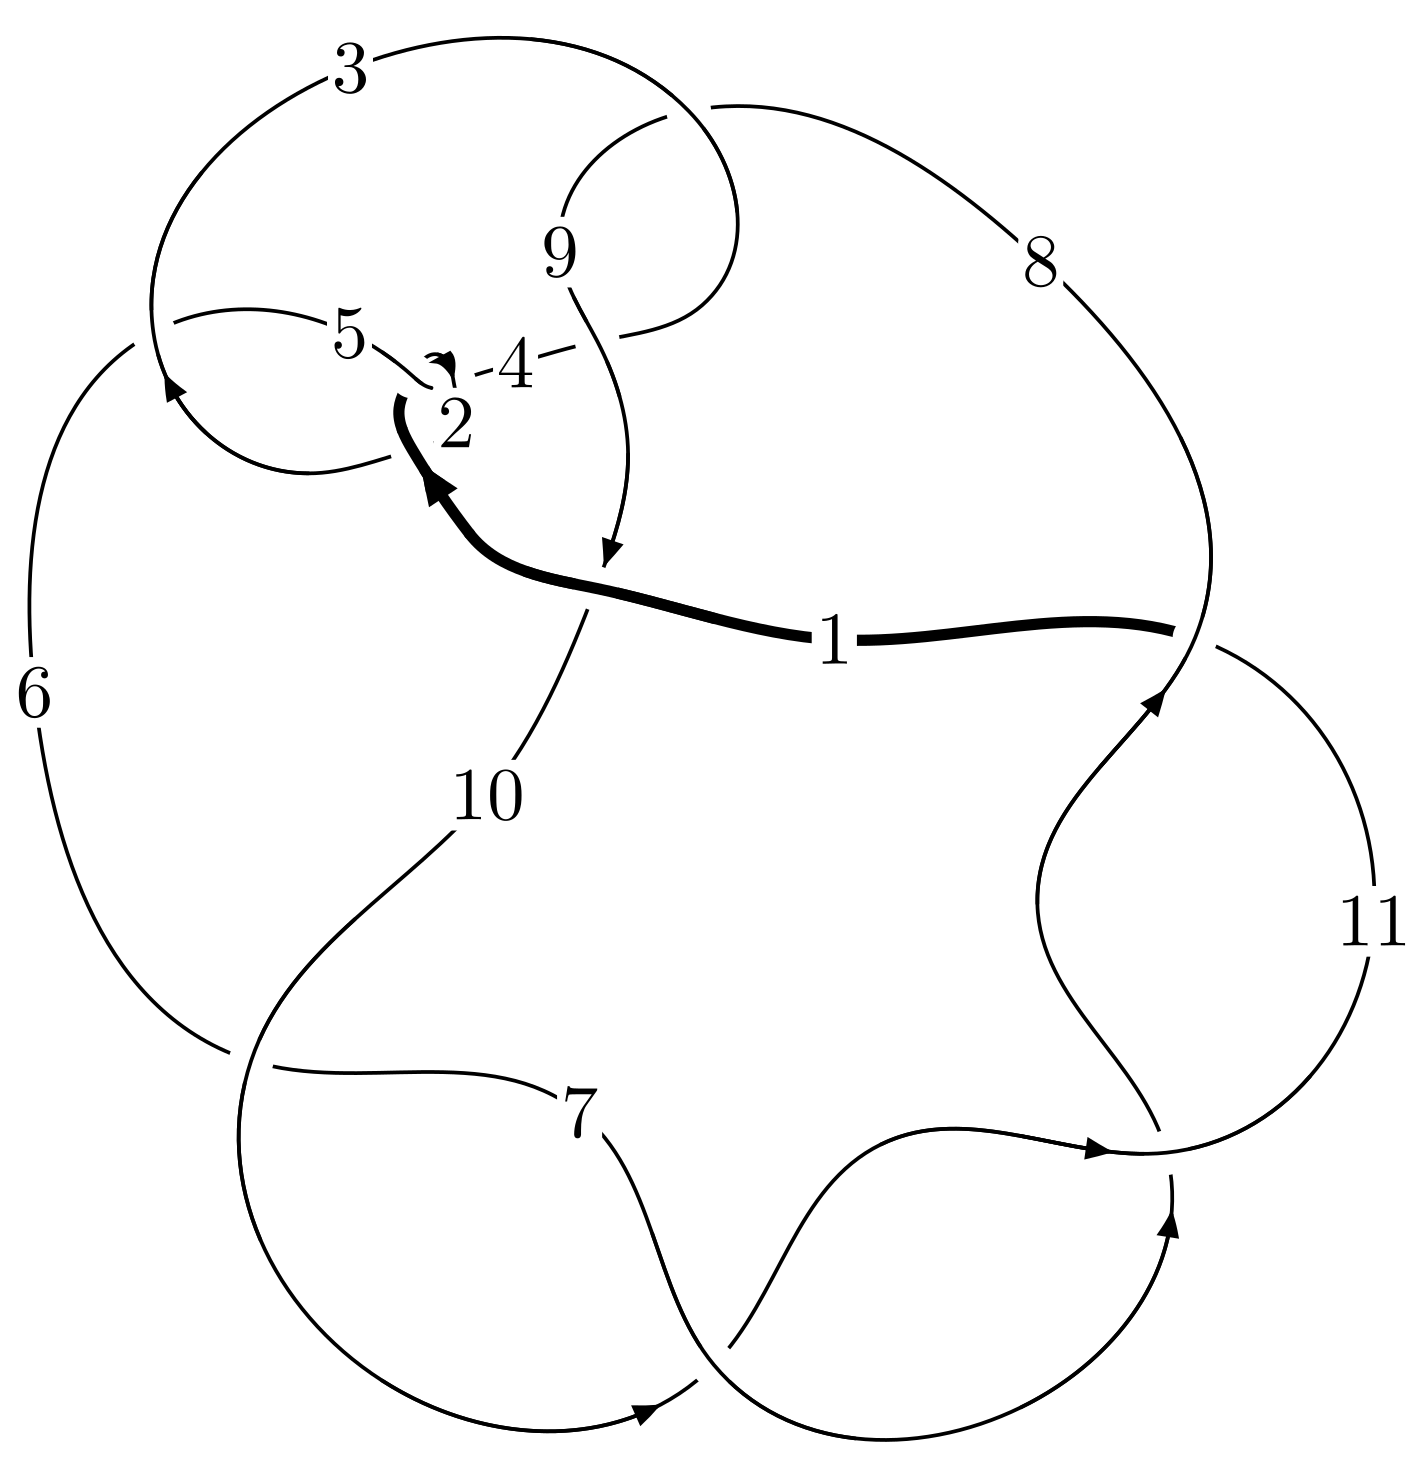
\includegraphics[width=112pt]{../../../GIT/diagram.site/Diagrams/png/631_11n_15.png}\\
\ \ \ A knot diagram\footnotemark}&
\allowdisplaybreaks
\textbf{Linearized knot diagam} \\
\cline{2-2}
 &
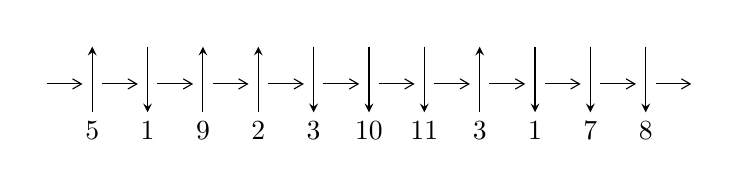
\begin{tikzpicture}[x=20pt, y=17pt]
	% nodes
	\node (C0) at (0, 0) {};
	\node (C1) at (1, 0) {};
	\node (C1U) at (1, +1) {};
	\node (C1D) at (1, -1) {5};

	\node (C2) at (2, 0) {};
	\node (C2U) at (2, +1) {};
	\node (C2D) at (2, -1) {1};

	\node (C3) at (3, 0) {};
	\node (C3U) at (3, +1) {};
	\node (C3D) at (3, -1) {9};

	\node (C4) at (4, 0) {};
	\node (C4U) at (4, +1) {};
	\node (C4D) at (4, -1) {2};

	\node (C5) at (5, 0) {};
	\node (C5U) at (5, +1) {};
	\node (C5D) at (5, -1) {3};

	\node (C6) at (6, 0) {};
	\node (C6U) at (6, +1) {};
	\node (C6D) at (6, -1) {10};

	\node (C7) at (7, 0) {};
	\node (C7U) at (7, +1) {};
	\node (C7D) at (7, -1) {11};

	\node (C8) at (8, 0) {};
	\node (C8U) at (8, +1) {};
	\node (C8D) at (8, -1) {3};

	\node (C9) at (9, 0) {};
	\node (C9U) at (9, +1) {};
	\node (C9D) at (9, -1) {1};

	\node (C10) at (10, 0) {};
	\node (C10U) at (10, +1) {};
	\node (C10D) at (10, -1) {7};

	\node (C11) at (11, 0) {};
	\node (C11U) at (11, +1) {};
	\node (C11D) at (11, -1) {8};
	\node (C12) at (12, 0) {};

	% arrows
	\draw[->,>={angle 60}]
	(C0) edge (C1) (C1) edge (C2) (C2) edge (C3) (C3) edge (C4) (C4) edge (C5) (C5) edge (C6) (C6) edge (C7) (C7) edge (C8) (C8) edge (C9) (C9) edge (C10) (C10) edge (C11) (C11) edge (C12) ;	\draw[->,>=stealth]
	(C1D) edge (C1U) (C2U) edge (C2D) (C3D) edge (C3U) (C4D) edge (C4U) (C5U) edge (C5D) (C6U) edge (C6D) (C7U) edge (C7D) (C8D) edge (C8U) (C9U) edge (C9D) (C10U) edge (C10D) (C11U) edge (C11D) ;
	\end{tikzpicture} \\
\hhline{~~} \\& 
\textbf{Solving Sequence} \\ \cline{2-2} 
 &
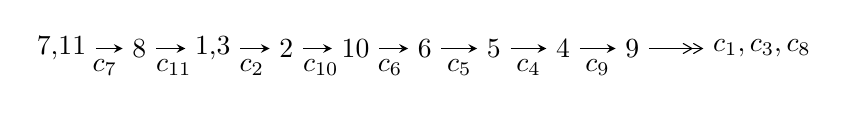
\begin{tikzpicture}[x=25pt, y=7pt]
	% node
	\node (A0) at (-1/8, 0) {7,11};
	\node (A1) at (1, 0) {8};
	\node (A2) at (33/16, 0) {1,3};
	\node (A3) at (25/8, 0) {2};
	\node (A4) at (33/8, 0) {10};
	\node (A5) at (41/8, 0) {6};
	\node (A6) at (49/8, 0) {5};
	\node (A7) at (57/8, 0) {4};
	\node (A8) at (65/8, 0) {9};
	\node (C1) at (1/2, -1) {$c_{7}$};
	\node (C2) at (3/2, -1) {$c_{11}$};
	\node (C3) at (21/8, -1) {$c_{2}$};
	\node (C4) at (29/8, -1) {$c_{10}$};
	\node (C5) at (37/8, -1) {$c_{6}$};
	\node (C6) at (45/8, -1) {$c_{5}$};
	\node (C7) at (53/8, -1) {$c_{4}$};
	\node (C8) at (61/8, -1) {$c_{9}$};
	\node (A9) at (10, 0) {$c_{1},c_{3},c_{8}$};

	% edge
	\draw[->,>=stealth]	
	(A0) edge (A1) (A1) edge (A2) (A2) edge (A3) (A3) edge (A4) (A4) edge (A5) (A5) edge (A6) (A6) edge (A7) (A7) edge (A8) ;
	\draw[->>,>={angle 60}]	
	(A8) edge (A9);
\end{tikzpicture} \\ 

\end{tabular} \\

\footnotetext{
The image of knot diagram is generated by the software ``\textbf{Draw programme}" developed by Andrew Bartholomew(\url{http://www.layer8.co.uk/maths/draw/index.htm\#Running-draw}), where we modified some parts for our purpose(\url{https://github.com/CATsTAILs/LinksPainter}).
}\phantom \\ \newline 
\centering \textbf{Ideals for irreducible components\footnotemark of $X_{\text{par}}$} 
 
\begin{align*}
I^u_{1}&=\langle 
3 u^{20}-5 u^{19}+\cdots+2 b+1,\;4 u^{20}-7 u^{19}+\cdots+2 a+1,\;u^{21}-3 u^{20}+\cdots- u-1\rangle \\
I^u_{2}&=\langle 
a u+b- a,\;a^2+a u+a+u+2,\;u^2+u-1\rangle \\
\\
\end{align*}
\raggedright * 2 irreducible components of $\dim_{\mathbb{C}}=0$, with total 25 representations.\\
\footnotetext{All coefficients of polynomials are rational numbers. But the coefficients are sometimes approximated in decimal forms when there is not enough margin.}
\newpage
\renewcommand{\arraystretch}{1}
\centering \section*{I. $I^u_{1}= \langle 3 u^{20}-5 u^{19}+\cdots+2 b+1,\;4 u^{20}-7 u^{19}+\cdots+2 a+1,\;u^{21}-3 u^{20}+\cdots- u-1 \rangle$}
\flushleft \textbf{(i) Arc colorings}\\
\begin{tabular}{m{7pt} m{180pt} m{7pt} m{180pt} }
\flushright $a_{7}=$&$\begin{pmatrix}1\\0\end{pmatrix}$ \\
\flushright $a_{11}=$&$\begin{pmatrix}0\\u\end{pmatrix}$ \\
\flushright $a_{8}=$&$\begin{pmatrix}1\\u^2\end{pmatrix}$ \\
\flushright $a_{1}=$&$\begin{pmatrix}- u\\- u^3+u\end{pmatrix}$ \\
\flushright $a_{3}=$&$\begin{pmatrix}-2 u^{20}+\frac{7}{2} u^{19}+\cdots-4 u-\frac{1}{2}\\-\frac{3}{2} u^{20}+\frac{5}{2} u^{19}+\cdots-\frac{3}{2} u-\frac{1}{2}\end{pmatrix}$ \\
\flushright $a_{2}=$&$\begin{pmatrix}-\frac{3}{2} u^{20}+2 u^{19}+\cdots+2 u^2-\frac{7}{2} u\\-\frac{5}{2} u^{20}+4 u^{19}+\cdots-\frac{3}{2} u-1\end{pmatrix}$ \\
\flushright $a_{10}=$&$\begin{pmatrix}u\\u\end{pmatrix}$ \\
\flushright $a_{6}=$&$\begin{pmatrix}- u^2+1\\- u^2\end{pmatrix}$ \\
\flushright $a_{5}=$&$\begin{pmatrix}\frac{1}{2} u^{19}- u^{18}+\cdots+3 u+\frac{1}{2}\\\frac{1}{2} u^{20}-\frac{1}{2} u^{19}+\cdots+\frac{3}{2} u+\frac{1}{2}\end{pmatrix}$ \\
\flushright $a_{4}=$&$\begin{pmatrix}-4 u^{20}+\frac{11}{2} u^{19}+\cdots-3 u-\frac{7}{2}\\-\frac{13}{2} u^{20}+\frac{21}{2} u^{19}+\cdots-\frac{15}{2} u-\frac{9}{2}\end{pmatrix}$ \\
\flushright $a_{9}=$&$\begin{pmatrix}- u^5+2 u^3+u\\- u^7+3 u^5-2 u^3+u\end{pmatrix}$\\ \flushright $a_{9}=$&$\begin{pmatrix}- u^5+2 u^3+u\\- u^7+3 u^5-2 u^3+u\end{pmatrix}$\\&\end{tabular}
\flushleft \textbf{(ii) Obstruction class $= -1$}\\~\\
\flushleft \textbf{(iii) Cusp Shapes $= \frac{13}{2} u^{20}-11 u^{19}-57 u^{18}+87 u^{17}+209 u^{16}-\frac{459}{2} u^{15}-462 u^{14}+\frac{319}{2} u^{13}+\frac{1465}{2} u^{12}+258 u^{11}-713 u^{10}-\frac{1001}{2} u^9+174 u^8+353 u^7+160 u^6-101 u^5+\frac{9}{2} u^4-77 u^3+13 u^2-\frac{1}{2} u+4$}\\~\\
\newpage\renewcommand{\arraystretch}{1}
\flushleft \textbf{(iv) u-Polynomials at the component}\newline \\
\begin{tabular}{m{50pt}|m{274pt}}
Crossings & \hspace{64pt}u-Polynomials at each crossing \\
\hline $$\begin{aligned}c_{1},c_{4}\end{aligned}$$&$\begin{aligned}
&u^{21}+3 u^{20}+\cdots- u-1
\end{aligned}$\\
\hline $$\begin{aligned}c_{2}\end{aligned}$$&$\begin{aligned}
&u^{21}+5 u^{20}+\cdots-13 u-1
\end{aligned}$\\
\hline $$\begin{aligned}c_{3},c_{8}\end{aligned}$$&$\begin{aligned}
&u^{21}- u^{20}+\cdots+16 u+16
\end{aligned}$\\
\hline $$\begin{aligned}c_{5}\end{aligned}$$&$\begin{aligned}
&u^{21}-3 u^{20}+\cdots-517 u-241
\end{aligned}$\\
\hline $$\begin{aligned}c_{6},c_{7},c_{10}\\c_{11}\end{aligned}$$&$\begin{aligned}
&u^{21}+3 u^{20}+\cdots- u+1
\end{aligned}$\\
\hline $$\begin{aligned}c_{9}\end{aligned}$$&$\begin{aligned}
&u^{21}- u^{20}+\cdots+3 u+1
\end{aligned}$\\
\hline
\end{tabular}\\~\\
\newpage\renewcommand{\arraystretch}{1}
\flushleft \textbf{(v) Riley Polynomials at the component}\newline \\
\begin{tabular}{m{50pt}|m{274pt}}
Crossings & \hspace{64pt}Riley Polynomials at each crossing \\
\hline $$\begin{aligned}c_{1},c_{4}\end{aligned}$$&$\begin{aligned}
&y^{21}+5 y^{20}+\cdots-13 y-1
\end{aligned}$\\
\hline $$\begin{aligned}c_{2}\end{aligned}$$&$\begin{aligned}
&y^{21}+25 y^{20}+\cdots+31 y-1
\end{aligned}$\\
\hline $$\begin{aligned}c_{3},c_{8}\end{aligned}$$&$\begin{aligned}
&y^{21}-25 y^{20}+\cdots+1408 y-256
\end{aligned}$\\
\hline $$\begin{aligned}c_{5}\end{aligned}$$&$\begin{aligned}
&y^{21}+45 y^{20}+\cdots-1228357 y-58081
\end{aligned}$\\
\hline $$\begin{aligned}c_{6},c_{7},c_{10}\\c_{11}\end{aligned}$$&$\begin{aligned}
&y^{21}-23 y^{20}+\cdots- y-1
\end{aligned}$\\
\hline $$\begin{aligned}c_{9}\end{aligned}$$&$\begin{aligned}
&y^{21}+37 y^{20}+\cdots- y-1
\end{aligned}$\\
\hline
\end{tabular}\\~\\
\newpage\flushleft \textbf{(vi) Complex Volumes and Cusp Shapes}
$$\begin{array}{c|c|c}  
\text{Solutions to }I^u_{1}& \I (\text{vol} + \sqrt{-1}CS) & \text{Cusp shape}\\
 \hline 
\begin{aligned}
u &= -0.586384 + 0.784633 I \\
a &= -0.273404 - 1.248180 I \\
b &= \phantom{-}0.731733 + 0.893746 I\end{aligned}
 & \phantom{-}9.06037 + 6.00997 I & -1.49297 - 4.91702 I \\ \hline\begin{aligned}
u &= -0.586384 - 0.784633 I \\
a &= -0.273404 + 1.248180 I \\
b &= \phantom{-}0.731733 - 0.893746 I\end{aligned}
 & \phantom{-}9.06037 - 6.00997 I & -1.49297 + 4.91702 I \\ \hline\begin{aligned}
u &= -0.502427 + 0.810890 I \\
a &= \phantom{-}0.300534 + 0.922223 I \\
b &= -1.209200 - 0.664376 I\end{aligned}
 & \phantom{-}9.31347 - 0.73158 I & -0.878702 - 0.143829 I \\ \hline\begin{aligned}
u &= -0.502427 - 0.810890 I \\
a &= \phantom{-}0.300534 - 0.922223 I \\
b &= -1.209200 + 0.664376 I\end{aligned}
 & \phantom{-}9.31347 + 0.73158 I & -0.878702 + 0.143829 I \\ \hline\begin{aligned}
u &= \phantom{-}1.30058\phantom{ +0.000000I} \\
a &= -0.779544\phantom{ +0.000000I} \\
b &= -0.0623998\phantom{ +0.000000I}\end{aligned}
 & -2.53925\phantom{ +0.000000I} & -3.24500\phantom{ +0.000000I} \\ \hline\begin{aligned}
u &= \phantom{-}0.650843 + 0.188135 I \\
a &= -0.679014 - 0.497949 I \\
b &= \phantom{-}0.257058 + 0.102289 I\end{aligned}
 & -1.259870 - 0.426532 I & -8.18330 + 0.83082 I \\ \hline\begin{aligned}
u &= \phantom{-}0.650843 - 0.188135 I \\
a &= -0.679014 + 0.497949 I \\
b &= \phantom{-}0.257058 - 0.102289 I\end{aligned}
 & -1.259870 + 0.426532 I & -8.18330 - 0.83082 I \\ \hline\begin{aligned}
u &= -1.349430 + 0.063463 I \\
a &= \phantom{-}0.17958 - 2.26263 I \\
b &= -0.08959 - 2.87750 I\end{aligned}
 & -3.34560 + 2.92064 I & -6.05745 - 2.89789 I \\ \hline\begin{aligned}
u &= -1.349430 - 0.063463 I \\
a &= \phantom{-}0.17958 + 2.26263 I \\
b &= -0.08959 + 2.87750 I\end{aligned}
 & -3.34560 - 2.92064 I & -6.05745 + 2.89789 I \\ \hline\begin{aligned}
u &= \phantom{-}1.45264 + 0.09803 I \\
a &= \phantom{-}0.354434 - 0.632200 I \\
b &= -0.288153 - 1.061360 I\end{aligned}
 & -6.20743 - 3.92323 I & -7.50265 + 3.86571 I\\
 \hline 
 \end{array}$$\newpage$$\begin{array}{c|c|c}  
\text{Solutions to }I^u_{1}& \I (\text{vol} + \sqrt{-1}CS) & \text{Cusp shape}\\
 \hline 
\begin{aligned}
u &= \phantom{-}1.45264 - 0.09803 I \\
a &= \phantom{-}0.354434 + 0.632200 I \\
b &= -0.288153 + 1.061360 I\end{aligned}
 & -6.20743 + 3.92323 I & -7.50265 - 3.86571 I \\ \hline\begin{aligned}
u &= \phantom{-}1.51579 + 0.30268 I \\
a &= -1.36198 + 1.35966 I \\
b &= -2.52269 + 1.32132 I\end{aligned}
 & \phantom{-}2.78944 - 3.34833 I & -3.65691 + 0.92294 I \\ \hline\begin{aligned}
u &= \phantom{-}1.51579 - 0.30268 I \\
a &= -1.36198 - 1.35966 I \\
b &= -2.52269 - 1.32132 I\end{aligned}
 & \phantom{-}2.78944 + 3.34833 I & -3.65691 - 0.92294 I \\ \hline\begin{aligned}
u &= \phantom{-}0.033690 + 0.433118 I \\
a &= -1.030760 - 0.710959 I \\
b &= -0.333491 + 0.730890 I\end{aligned}
 & \phantom{-}0.87590 - 1.40870 I & \phantom{-}1.21226 + 3.90536 I \\ \hline\begin{aligned}
u &= \phantom{-}0.033690 - 0.433118 I \\
a &= -1.030760 + 0.710959 I \\
b &= -0.333491 - 0.730890 I\end{aligned}
 & \phantom{-}0.87590 + 1.40870 I & \phantom{-}1.21226 - 3.90536 I \\ \hline\begin{aligned}
u &= \phantom{-}1.56509 + 0.27721 I \\
a &= \phantom{-}1.22824 - 1.65327 I \\
b &= \phantom{-}2.69420 - 2.24461 I\end{aligned}
 & \phantom{-}2.01164 - 9.94805 I & -4.72572 + 5.38300 I \\ \hline\begin{aligned}
u &= \phantom{-}1.56509 - 0.27721 I \\
a &= \phantom{-}1.22824 + 1.65327 I \\
b &= \phantom{-}2.69420 + 2.24461 I\end{aligned}
 & \phantom{-}2.01164 + 9.94805 I & -4.72572 - 5.38300 I \\ \hline\begin{aligned}
u &= -0.317530 + 0.257874 I \\
a &= \phantom{-}2.02998 - 0.42048 I \\
b &= \phantom{-}0.636210 - 0.403748 I\end{aligned}
 & -0.37325 + 2.55975 I & \phantom{-}0.64804 - 6.58188 I \\ \hline\begin{aligned}
u &= -0.317530 - 0.257874 I \\
a &= \phantom{-}2.02998 + 0.42048 I \\
b &= \phantom{-}0.636210 + 0.403748 I\end{aligned}
 & -0.37325 - 2.55975 I & \phantom{-}0.64804 + 6.58188 I \\ \hline\begin{aligned}
u &= -1.61257 + 0.03861 I \\
a &= \phantom{-}0.642150 - 0.779274 I \\
b &= \phantom{-}1.15512 - 1.57833 I\end{aligned}
 & -9.12765 + 1.23257 I & -9.74011 + 3.00809 I\\
 \hline 
 \end{array}$$\newpage$$\begin{array}{c|c|c}  
\text{Solutions to }I^u_{1}& \I (\text{vol} + \sqrt{-1}CS) & \text{Cusp shape}\\
 \hline 
\begin{aligned}
u &= -1.61257 - 0.03861 I \\
a &= \phantom{-}0.642150 + 0.779274 I \\
b &= \phantom{-}1.15512 + 1.57833 I\end{aligned}
 & -9.12765 - 1.23257 I & -9.74011 - 3.00809 I\\
 \hline 
 \end{array}$$\newpage\newpage\renewcommand{\arraystretch}{1}
\centering \section*{II. $I^u_{2}= \langle a u+b- a,\;a^2+a u+a+u+2,\;u^2+u-1 \rangle$}
\flushleft \textbf{(i) Arc colorings}\\
\begin{tabular}{m{7pt} m{180pt} m{7pt} m{180pt} }
\flushright $a_{7}=$&$\begin{pmatrix}1\\0\end{pmatrix}$ \\
\flushright $a_{11}=$&$\begin{pmatrix}0\\u\end{pmatrix}$ \\
\flushright $a_{8}=$&$\begin{pmatrix}1\\- u+1\end{pmatrix}$ \\
\flushright $a_{1}=$&$\begin{pmatrix}- u\\- u+1\end{pmatrix}$ \\
\flushright $a_{3}=$&$\begin{pmatrix}a\\- a u+a\end{pmatrix}$ \\
\flushright $a_{2}=$&$\begin{pmatrix}- a u+2 a\\-3 a u+2 a\end{pmatrix}$ \\
\flushright $a_{10}=$&$\begin{pmatrix}u\\u\end{pmatrix}$ \\
\flushright $a_{6}=$&$\begin{pmatrix}u\\u-1\end{pmatrix}$ \\
\flushright $a_{5}=$&$\begin{pmatrix}a+2 u+1\\- a u+a+2 u-1\end{pmatrix}$ \\
\flushright $a_{4}=$&$\begin{pmatrix}a\\- a u+a\end{pmatrix}$ \\
\flushright $a_{9}=$&$\begin{pmatrix}1\\- u+1\end{pmatrix}$\\ \flushright $a_{9}=$&$\begin{pmatrix}1\\- u+1\end{pmatrix}$\\&\end{tabular}
\flushleft \textbf{(ii) Obstruction class $= 1$}\\~\\
\flushleft \textbf{(iii) Cusp Shapes $= -5 a u+2 a+u-8$}\\~\\
\newpage\renewcommand{\arraystretch}{1}
\flushleft \textbf{(iv) u-Polynomials at the component}\newline \\
\begin{tabular}{m{50pt}|m{274pt}}
Crossings & \hspace{64pt}u-Polynomials at each crossing \\
\hline $$\begin{aligned}c_{1},c_{2},c_{5}\end{aligned}$$&$\begin{aligned}
&(u^2+u+1)^2
\end{aligned}$\\
\hline $$\begin{aligned}c_{3},c_{8}\end{aligned}$$&$\begin{aligned}
&u^4
\end{aligned}$\\
\hline $$\begin{aligned}c_{4}\end{aligned}$$&$\begin{aligned}
&(u^2- u+1)^2
\end{aligned}$\\
\hline $$\begin{aligned}c_{6},c_{7},c_{9}\end{aligned}$$&$\begin{aligned}
&(u^2+u-1)^2
\end{aligned}$\\
\hline $$\begin{aligned}c_{10},c_{11}\end{aligned}$$&$\begin{aligned}
&(u^2- u-1)^2
\end{aligned}$\\
\hline
\end{tabular}\\~\\
\newpage\renewcommand{\arraystretch}{1}
\flushleft \textbf{(v) Riley Polynomials at the component}\newline \\
\begin{tabular}{m{50pt}|m{274pt}}
Crossings & \hspace{64pt}Riley Polynomials at each crossing \\
\hline $$\begin{aligned}c_{1},c_{2},c_{4}\\c_{5}\end{aligned}$$&$\begin{aligned}
&(y^2+y+1)^2
\end{aligned}$\\
\hline $$\begin{aligned}c_{3},c_{8}\end{aligned}$$&$\begin{aligned}
&y^4
\end{aligned}$\\
\hline $$\begin{aligned}c_{6},c_{7},c_{9}\\c_{10},c_{11}\end{aligned}$$&$\begin{aligned}
&(y^2-3 y+1)^2
\end{aligned}$\\
\hline
\end{tabular}\\~\\
\newpage\flushleft \textbf{(vi) Complex Volumes and Cusp Shapes}
$$\begin{array}{c|c|c}  
\text{Solutions to }I^u_{2}& \I (\text{vol} + \sqrt{-1}CS) & \text{Cusp shape}\\
 \hline 
\begin{aligned}
u &= \phantom{-}0.618034\phantom{ +0.000000I} \\
a &= -0.80902 + 1.40126 I \\
b &= -0.309017 + 0.535233 I\end{aligned}
 & -0.98696 + 2.02988 I & -6.50000 - 1.52761 I \\ \hline\begin{aligned}
u &= \phantom{-}0.618034\phantom{ +0.000000I} \\
a &= -0.80902 - 1.40126 I \\
b &= -0.309017 - 0.535233 I\end{aligned}
 & -0.98696 - 2.02988 I & -6.50000 + 1.52761 I \\ \hline\begin{aligned}
u &= -1.61803\phantom{ +0.000000I} \\
a &= \phantom{-}0.309017 + 0.535233 I \\
b &= \phantom{-}0.80902 + 1.40126 I\end{aligned}
 & -8.88264 - 2.02988 I & -6.50000 + 5.40059 I \\ \hline\begin{aligned}
u &= -1.61803\phantom{ +0.000000I} \\
a &= \phantom{-}0.309017 - 0.535233 I \\
b &= \phantom{-}0.80902 - 1.40126 I\end{aligned}
 & -8.88264 + 2.02988 I & -6.50000 - 5.40059 I\\
 \hline 
 \end{array}$$\newpage
\newpage\renewcommand{\arraystretch}{1}
\centering \section*{ III. u-Polynomials}
\begin{tabular}{m{50pt}|m{274pt}}
Crossings & \hspace{64pt}u-Polynomials at each crossing \\
\hline $$\begin{aligned}c_{1}\end{aligned}$$&$\begin{aligned}
&((u^2+u+1)^2)(u^{21}+3 u^{20}+\cdots- u-1)
\end{aligned}$\\
\hline $$\begin{aligned}c_{2}\end{aligned}$$&$\begin{aligned}
&((u^2+u+1)^2)(u^{21}+5 u^{20}+\cdots-13 u-1)
\end{aligned}$\\
\hline $$\begin{aligned}c_{3},c_{8}\end{aligned}$$&$\begin{aligned}
&u^4(u^{21}- u^{20}+\cdots+16 u+16)
\end{aligned}$\\
\hline $$\begin{aligned}c_{4}\end{aligned}$$&$\begin{aligned}
&((u^2- u+1)^2)(u^{21}+3 u^{20}+\cdots- u-1)
\end{aligned}$\\
\hline $$\begin{aligned}c_{5}\end{aligned}$$&$\begin{aligned}
&((u^2+u+1)^2)(u^{21}-3 u^{20}+\cdots-517 u-241)
\end{aligned}$\\
\hline $$\begin{aligned}c_{6},c_{7}\end{aligned}$$&$\begin{aligned}
&((u^2+u-1)^2)(u^{21}+3 u^{20}+\cdots- u+1)
\end{aligned}$\\
\hline $$\begin{aligned}c_{9}\end{aligned}$$&$\begin{aligned}
&((u^2+u-1)^2)(u^{21}- u^{20}+\cdots+3 u+1)
\end{aligned}$\\
\hline $$\begin{aligned}c_{10},c_{11}\end{aligned}$$&$\begin{aligned}
&((u^2- u-1)^2)(u^{21}+3 u^{20}+\cdots- u+1)
\end{aligned}$\\
\hline
\end{tabular}\newpage\renewcommand{\arraystretch}{1}
\centering \section*{ IV. Riley Polynomials}
\begin{tabular}{m{50pt}|m{274pt}}
Crossings & \hspace{64pt}Riley Polynomials at each crossing \\
\hline $$\begin{aligned}c_{1},c_{4}\end{aligned}$$&$\begin{aligned}
&((y^2+y+1)^2)(y^{21}+5 y^{20}+\cdots-13 y-1)
\end{aligned}$\\
\hline $$\begin{aligned}c_{2}\end{aligned}$$&$\begin{aligned}
&((y^2+y+1)^2)(y^{21}+25 y^{20}+\cdots+31 y-1)
\end{aligned}$\\
\hline $$\begin{aligned}c_{3},c_{8}\end{aligned}$$&$\begin{aligned}
&y^4(y^{21}-25 y^{20}+\cdots+1408 y-256)
\end{aligned}$\\
\hline $$\begin{aligned}c_{5}\end{aligned}$$&$\begin{aligned}
&((y^2+y+1)^2)(y^{21}+45 y^{20}+\cdots-1228357 y-58081)
\end{aligned}$\\
\hline $$\begin{aligned}c_{6},c_{7},c_{10}\\c_{11}\end{aligned}$$&$\begin{aligned}
&((y^2-3 y+1)^2)(y^{21}-23 y^{20}+\cdots- y-1)
\end{aligned}$\\
\hline $$\begin{aligned}c_{9}\end{aligned}$$&$\begin{aligned}
&((y^2-3 y+1)^2)(y^{21}+37 y^{20}+\cdots- y-1)
\end{aligned}$\\
\hline
\end{tabular}
\vskip 2pc
\end{document}